
\begin{lead}
 ある一定の数式にて与えられる信号波形に対してはフーリエ係数を計算でき,周波数領域においては信号の性質を調査することができる.しかし,実際に観測される信号は関数で表現されることがまれであり,表現できたとしても,それはあくまでも近似的な数式である.

 離散化されたディジタル信号であっても,フーリエ係数が求められれば,大変便利である.これは離散フーリエ変換 (Discrete Fourier Transform: DFT)によって実現されるのである.
%
本章では,離散フーリエ変換の扱いについて学ぶ.


\end{lead}

%\vfill

%\begin{koumoku}
%#集合\\
%#離散集合\\
%#部分集合と包含関係\\
%#ベキ集合\\
%#集合演算\\
%#集合演算の性質\\
%#包除原理\\
%#集合の直和と直和分割\\
%#集合の直積
%#\end{koumoku}

%#\clearpage

\chapter{離散フーリエ変換}

\label{chapter:dft}


\section{離散フーリエ変換の式}

もし,$x(t)$が周期$T$による\index{しゅうきかんすう@周期関数}周期関数である場合,$x(t)$の\index{ふーりえきゅうすうてんかい@フーリエ級数展開}フーリエ級数展開式は,次式のように表される.
\begin{equation}
x(t)=\sum^{\infty}_{k=-\infty}C_k e^{j\omega t}
\label{eqn:invdft1}
\end{equation}
ただし,$\omega$は,
\begin{equation}
\omega = \frac{2\pi}{T}
\end{equation}
である.また,\index{ふーりえけいすう@フーリエ係数}フーリエ係数$C_k$は,
\begin{equation}
C_k = \frac{1}{T} \int^{T/2}_{-T/2} x(t) e^{-jk\omega t}dt
\label{eqn:fourier-keisu-dft1}
\end{equation}
である.いま,図\ref{fig:shuki-singou1}に示すように,$x(t)$が等間隔$\tau$で\index{さんぷりんぐ@サンプリング}サンプリングされた$N$個の\index{さんぷりんぐでーた@サンプリングデータ}サンプリングデータで与えられている場合を考える.

\begin{figure}[H]
\begin{center}
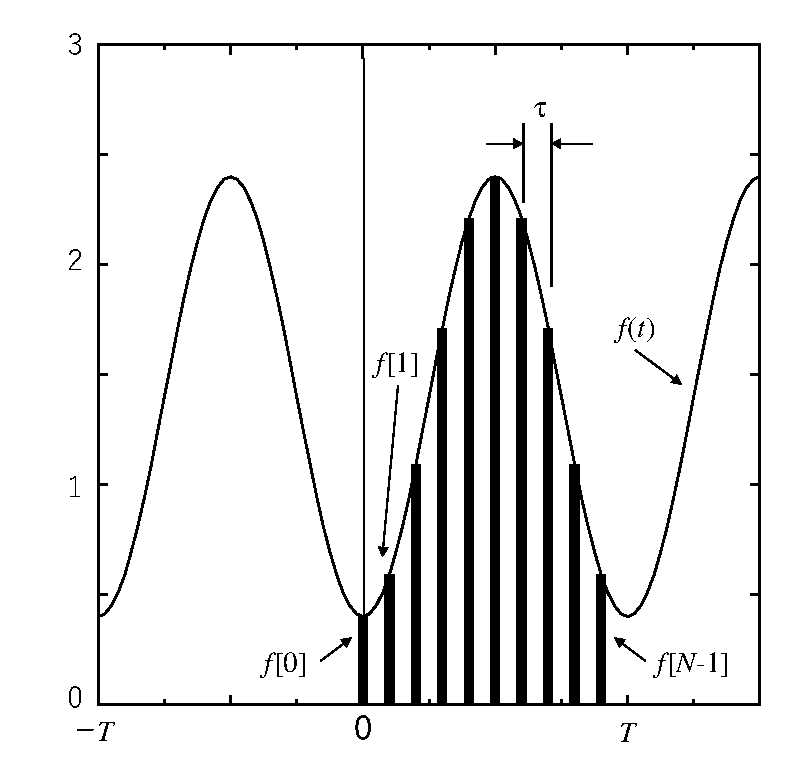
\includegraphics[width=.65\textwidth]{fig/shuki-sample-1.eps}
\caption{周期信号のサンプリングデータ}
\end{center}
\label{fig:shuki-singou1}
\end{figure}

基本区間を$[0,T]$とすると,サンプリング点は,
\begin{equation}
t_i=i\tau=\frac{iT}{N} \hspace{1cm} (i=0,1,2,\ldots,N-1)
\end{equation}
と書くことができ
\footnote{
%\begin{eqnarray}
$\displaystyle \omega t_i = \frac{2\pi}{T} \cdot i \frac{T}{N} %\nonumber \\
 = \frac{2\pi i}{N}$
%\end{eqnarray},
%\begin{equation}
$\displaystyle \tau=\frac{T}{N}$
%\end{equation}
を用いる.
}
,サンプリングデータは
\begin{equation}
x[i]=x \left ( \frac{iT}{N} \right ) \hspace{1cm} (i=0,1,2,\ldots,N-1)
\end{equation}
である.

ところで,離散化された$x[i]$に対して,式(\ref{eqn:fourier-keisu-dft1})の積分は,次式のような積和の形式で書くことができる.
%&\footnote{
\begin{equation}
C_k = \frac{1}{T} \sum^{N-1}_{i=0} x[i] e^{-jk\omega t_i} \tau %\nonumber \\
 = \frac{1}{N} \sum^{N-1}_{i=0} x[i] e^{-j\frac{2\pi}{N}ki}
\label{eqn:fourier-keisu-dft2}
\end{equation}
%}
%
この式(\ref{eqn:fourier-keisu-dft2})を\index{りさんふーりえへんかん@離散フーリエ変換}離散フーリエ変換と呼ぶ.ここで,連続信号に対するフーリエ係数が無限に発生するにもかかわらず,離散フーリエ変換ではデータの個数は$N$個であることに注意する必要がある.

実際には,式(\ref{eqn:fourier-keisu-dft2})から無限個の$C_k$が計算できるが,後述のような周期性により,データの個数は$N$個で十分であるといえる.式(\ref{eqn:fourier-keisu-dft2})の逆変換は,式(\ref{eqn:invdft1})を直接離散化すればよく,
\begin{equation}
x[i] = \sum^{N-1}_{i=0} C_k e^{j\frac{2\pi}{N}ki} \hspace{5mm} (i=0,1,2,\ldots,N-1)
\label{eqn:fourier-keisu-dft3}
\end{equation}
を\index{りさんふーりえぎゃくへんかん@離散フーリエ逆変換}離散フーリエ逆変換 (Inverse Discrete Fourier Transform: IDFT) と呼ばれる.これも積和の個数は$N$個である.

ところで,式(\ref{eqn:fourier-keisu-dft2})には$1/N$があるが,式(\ref{eqn:fourier-keisu-dft3})には$1/N$が付いていない.式(\ref{eqn:fourier-keisu-dft2})の$1/N$は$N$の増加とともに$C_k$の値が大きくなることを避けるために必要なものである
\footnote{式(\ref{eqn:fourier-keisu-dft2})に$1/N$がついておらず,式(\ref{eqn:fourier-keisu-dft3})に$1/N$が付いていてもよい.また,式(\ref{eqn:fourier-keisu-dft2})に$1/\sqrt{N}$がついていて,式(\ref{eqn:fourier-keisu-dft3})にも$1/\sqrt{N}$が付いていてもよいのである.}.

続いて,DFTを計算する場合に,ここまで指数関数での表記をしたが,三角関数による表記を考える.オイラーの公式
\footnote{オイラーの公式は$e^{j\theta}=\cos \theta +j \sin \theta$と書くことができる.}
を用いると,式(\ref{eqn:fourier-keisu-dft2})は,

\begin{eqnarray}
C_k &=& \frac{1}{N} \sum^{N-1}_{i=0} x[i] \left \{ \cos \frac{2\pi}{N}ki -j \sin \frac{2\pi}{N}ki \right \} \nonumber \\
 &=& A_k + B_k
\label{eqn:fourier-keisu-dft4}
\end{eqnarray}\vskip.3\baselineskip

\noindent と書くことができる.ここで,

\begin{eqnarray}
A_k &=& \frac{1}{N} \sum^{N-1}_{i=0} x[i]  \cos \frac{2\pi}{N}ki \\
B_k &=& -\frac{1}{N} \sum^{N-1}_{i=0} x[i]  \sin \frac{2\pi}{N}ki
\label{eqn:fourier-keisu-dft5}
\end{eqnarray}\vskip.5\baselineskip

\noindent である.これを用いて,IDFTは式(\ref{eqn:fourier-keisu-dft3})より,以下のように書くことができる.

\begin{eqnarray}
x[i] &=& \sum^{N-1}_{i=0} C_k e^{j\frac{2\pi}{N}ki} \\
 &=& \sum^{N-1}_{i=0} (A_k + j B_k) \left ( \cos \frac{2\pi}{N}ki +j \sin \frac{2\pi}{N}ki \right ) \\
 &=& \sum^{N-1}_{i=0} \left ( A_k \cos \frac{2\pi}{N}ki + B_k \sin \frac{2\pi}{N}ki \right ) \nonumber \\
 & & +j \sum^{N-1}_{i=0} \left ( A_k \sin \frac{2\pi}{N}ki + B_k \cos \frac{2\pi}{N}ki \right ) \label{eqn:fourier-keisu-dft6} \\
 &=& \sum^{N-1}_{i=0} \left ( A_k \cos \frac{2\pi}{N}ki + B_k \sin \frac{2\pi}{N}ki \right ) 
\label{eqn:fourier-keisu-dft7}
\end{eqnarray}\vskip.3\baselineskip

なお,以下のように,式(\ref{eqn:fourier-keisu-dft6})の虚部は常に0となる.

\begin{eqnarray}
 & & \sum^{N-1}_{i=0} \left ( A_k \sin \frac{2\pi}{N}ki + B_k \cos \frac{2\pi}{N}ki \right ) \nonumber \\
 &=& \sum^{N-1}_{i=0} \left ( \sum^{N-1}_{i=0} x[i] (\cos \frac{2\pi}{N}ki \sin \frac{2\pi}{N}ki  - \sin \frac{2\pi}{N}ki \cos \frac{2\pi}{N}ki \right ) \nonumber \\
 &=& 0
\end{eqnarray}

\section{離散フーリエ変換の特徴}

離散フーリエ変換(DFT)によって得られた結果(FFTであっても結果は同じ)を理解する上で,解析的に得られるフーリエ係数の厳密解と,離散フーリエ変換によって得られた結果との差異を把握することが目的である.

\subsection{\index{すぺくとる@スペクトル}スペクトルの\index{しゅうきせい@周期性}周期性}

式(\ref{eqn:fourier-keisu-dft2})より,$N$個シフトしたフーリエ係数は,

\begin{eqnarray}
C_{k+N} &=& \frac{1}{T} \sum^{N-1}_{i=0} x[i] e^{-j\frac{2\pi}{N}(k+N) i} \nonumber \\
 &=& \frac{1}{T} \sum^{N-1}_{i=0} x[i] e^{-j\frac{2\pi}{N}ki} e^{-2j\pi i} \nonumber \\
 &=& \frac{1}{T} \sum^{N-1}_{i=0} x[i] e^{-j\frac{2\pi}{N}ki} \nonumber \\
 &=& C_k
\label{eqn:fourier-keisu-dft21}
\end{eqnarray}\vskip.3\baselineskip

\noindent となるので,\index{DFT@DFT}DFTによって得られるフーリエ係数は$N$の周期を持っている,ということができる.このことから,$C_k$は無限個計算することが可能であるが,それらは$k=0 \sim N-1$のいずれかと一致するので,データ数と同じ$N$個だけ計算すればよいのである.


\subsection{スペクトルの対称性}

式(\ref{eqn:fourier-keisu-dft2})より,DFTにおける負の次数 ($k=-1,-2,-3,\cdots$)のスペクトル(フーリエ係数)は,$N=8$であるとき,$k=7,6,5\cdots$に現れる.このことを一般式で示すと,


\begin{eqnarray}
C_{N-k} &=& \frac{1}{T} \sum^{N-1}_{i=0} x[i] e^{-j\frac{2\pi}{N}(N-k) i} \nonumber \\
 &=& \frac{1}{T} \sum^{N-1}_{i=0} x[i] e^{-j\frac{2\pi}{N}(-k)i} e^{-2j\pi i} \nonumber \\
 &=& \frac{1}{T} \sum^{N-1}_{i=0} x[i] e^{-j\frac{2\pi}{N}(-k)i} \nonumber \\
 &=& C_{-k}
\label{eqn:fourier-keisu-dft22}
\end{eqnarray}\vskip.3\baselineskip

\noindent となるので,DFTによって得られるフーリエ係数$C_k$の実数部については$k=0$を中心に,左右対称であり,虚数部については$k=0$を中心に点対称であることがわかる.


\subsection{DFTの計算例}

ここでは,実際に図\ref{fig:zu4-41}に示すような方形波に対してDFTを用いた計算を行う.DFTを用いる場合には,サンプリングを行う区間に$[-T/2,T/2]$ではなく$[0,T]$の領域を考えるものとする.また,不連続点では2点間の中心値を用いることとする.ここで,$N=8$のときのサンプリングデータは,次式のようになる.
\begin{equation}
x[i]=\{ 1, 1,0.5, 0, 0, 0, 0.5, 1 \}
\label{eqn:houkeiha_1}
\end{equation}

ここで,式(\ref{eqn:fourier-keisu-dft7})により$A_k$,$B_k$を求めると,$x[t]$は偶関数であることより,実数部だけとると考えることができる.
%
その結果について,解析解であれば,
\begin{equation}
C_k=\frac{t_w}{T} \mathrm{sinc} \left ( k \pi \frac{t_w}{T} \right )
\end{equation}
となるが,$t_w/T = 0.5$として求めることができる.なお,本章では$\tau$をサンプリング間隔,$t_w$をパルス幅の記号としている.

\begin{figure}[H]
\begin{center}
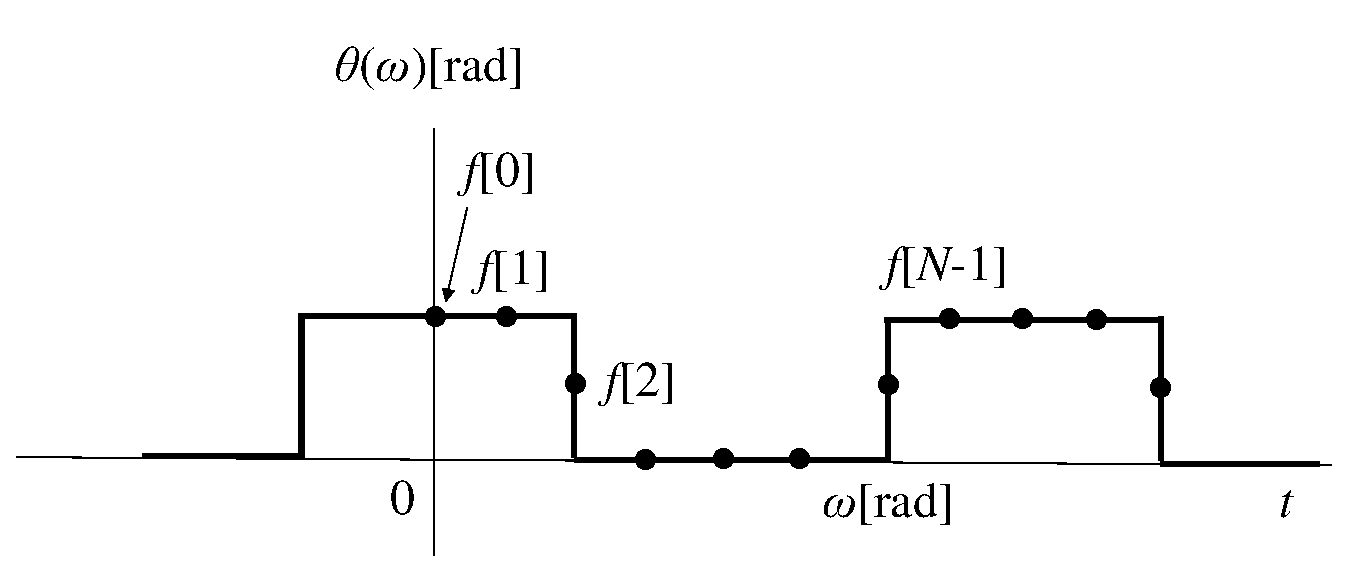
\includegraphics[width=.7\textwidth]{fig/zu-4-5.eps}
\end{center}
\caption{DFTを行うためのデータのとり方}
\label{fig:zu4-41}
\end{figure}

DFTの結果は図\ref{fig:zu4-51}のようになるが,$k=N/2$を中心に左右対称となり,$A_5$,$A_6$,$A_7$は解析解の$C_{-1}$,$C_{-2}$,$C_{-3}$に相当していることがわかる.すなわち,解析解と比較可能であるのは$k=0 \sim N/2$に対してだけである.

このように少ないサンプリング点数から成り立つサンプリングデータに対してでも,直流分は完全に一致し,基本は成分も一致していることがわかる.一般的に,$N/2$に近くなるほど誤差が大きくなる.

\begin{figure}[H]
\begin{center}
\begin{minipage}[b]{.58\textwidth}
\begin{center}
\includegraphics[height=3.5cm]{fig/zu-4-5a.eps}

(a) 解析解 ($N=8$)
\end{center}
\end{minipage}
\begin{minipage}[b]{.38\textwidth}
\begin{center}
\includegraphics[height=3.5cm]{fig/zu-4-5b.eps}

(b) DFT ($N=8$)
\end{center}
\end{minipage}
\end{center}\vskip.5\baselineskip
\caption{方形波に対するスペクトルの比較}
\label{fig:zu4-51}
\end{figure}

%\begin{table}[ht]
%\begin{center}
%\caption{方形波(式(\ref{eqn:houkeiha_1}))のスペクトルの計算例}
%\begin{tabular}{c|c|c|l}
%\hline
%k & 解析解 $\Re [C_k]$ & DFT $A_k$ & 意味 \\
%\hline
%0 & 0.5 & 0.5 & 解析解と比較可能 \\
%1 & $1/\pi$ & 0.3018 & 解析解と比較可能 \\
%2 & 0.0  & 0.0 & 解析解と比較可能 \\
%3 & $-1/3\pi$ & -0.0518 & 解析解と比較可能 \\
%4 & 0.0 & 0.0 & 解析解と比較可能 \\
%5 & $1/5\pi$ & -0.518 & $A_3$と同じ \\
%6 & 0.0 & 0.0 & $A_2$と同じ \\
%7 & $-1/7\pi$ & 0.3018 & $A_1$と同じ \\
%\hline
%\end{tabular}
%\end{center}
%\label{table:riron-kaiseki-9-3}
%\end{table}


\section*{演習問題}

\subsection*{問題\ref{chapter:dft}.1}

4点データ$x[0]=1$,$x[1]=1$,$x[2]=0$,$x[3]=1$に関する4点DFTを求めよ.

\subsection*{問題\ref{chapter:dft}.2}

$x(n)=\sin ( \omega_c n)$のDFTを$0 \leq k < N$の範囲で求めよ.ただし,$\omega_c=6\pi /N$,$N>3$とする.



